% !TEX encoding = UTF-8 Unicode
\documentclass[11pt, a4paper, oneside, onecolumn]{ctexart}
\usepackage[utf8]{inputenc}
\usepackage{geometry}
\geometry{left=1.5cm,right=1.5cm,top=2cm,bottom=1cm}
\usepackage{ctex}
\usepackage{CJK}
\usepackage{xcolor}

\usepackage{amsmath, amsthm, amssymb, graphicx, mathrsfs, siunitx}
\usepackage{tikz}
\usepackage{subfigure}
\usepackage{caption}
\usepackage{subcaption}
\usepackage[flushleft]{threeparttable}
\usepackage{cases}

\ctexset{section={format=\bfseries \zihao{4} \flushleft}}
\renewcommand\thesubsection{\thesection.\arabic{subsection}}
\numberwithin{equation}{subsection}
\renewcommand\theequation{\thesubsection.\arabic{equation}}
\makeatletter
\renewcommand{\maketag@@@}[1]{\hbox{\m@th\normalsize\normalfont#1}}%
\makeatother

\usepackage{bookmark}
\usepackage{hyperref}
\hypersetup{colorlinks=true,linkcolor=black}
\usepackage{indentfirst}
\usepackage{inconsolata}

\usepackage{listings}
\lstset{
     basicstyle      =   \zihao{-5}\ttfamily,
     numberstyle     =   \zihao{-5}\ttfamily,
     keywordstyle    =   \color{blue},
     keywordstyle    =   [2] \color{teal},
     stringstyle     =   \color{magenta},
     commentstyle    =   \color{red}\ttfamily,
     breaklines      =   true,   % 自动换行,建议不要写太长的行
     columns         =   fixed,  % 如果不加这一句,字间距就不固定
     flexiblecolumns,                % 别问为什么,加上这个
     numbers             =   left,   % 行号的位置在左边
     showspaces          =   false,  % 是否显示空格,显示了有点乱
     numberstyle         =   \zihao{-5}\ttfamily,    % 行号的样式,小五号,tt 等宽字体
     showstringspaces    =   false,
     captionpos          =   t,      % 这段代码的名字所呈现的位置,t 指的是 top 上面
     frame               =   lrtb,   % 显示边框
}

\lstdefinestyle{Python}{
     language        =   Python,
     basicstyle      =   \zihao{-5}\ttfamily,
     numberstyle     =   \zihao{-5}\ttfamily,
     keywordstyle    =   \color{blue},
     keywordstyle    =   [2] \color{teal},
     stringstyle     =   \color{magenta},
     commentstyle    =   \color{red}\ttfamily,
     breaklines      =   true,   % 自动换行,建议不要写太长的行
     columns         =   fixed,  % 如果不加这一句,字间距就不固定
basewidth       =   0.5em,
}

% \usepackage{physics} % 物理百宝箱
% \usepackage[version=4]{mhchem} % 绘制分子式
% \usepackage{algorithm,algorithmic} % 展示算法伪代码
\usepackage[backend=biber,sorting=none]{biblatex}
\addbibresource{/Users/Linyan/Zotero/MyBibTex.bib}

\title{实测天体物理}
\author{林衍}
\date{\today}

\begin{document}
\maketitle
\subsection*{前言}


\newpage
\tableofcontents

\newpage
\section{太阳}
黑子由本影与半影组成,温度约$3000\text{\textendash}4500\,\mathrm{K}$, 产生原因是黑子下方的强磁场$\left(\sim10^{3}\,\mathrm{G}\right)$阻碍了物质对流,使热量难以到达该处。

太阳内部等离子体转动产生磁场。由于对流区较差转动产生横向磁场。磁力线突出日面就形成黑子、日珥和耀斑。

太阳磁场的发电机理论:太阳内部等离子体的转动产生磁场:
\begin{equation}
\frac{\partial{}\boldsymbol{B}}{\partial{}t}=\nabla\times\left(\boldsymbol{u}\times\boldsymbol{B}-\eta\nabla\times\boldsymbol{B}\right),
\end{equation}
其中$\eta$是磁扩散系数。

太阳对流区具有较差转动的特点,一般认为环向磁场产生于辐射区和对流区的交界面差旋层。
\begin{figure}[!htbp]
\centering
\begin{minipage}[t]{0.45\textwidth}
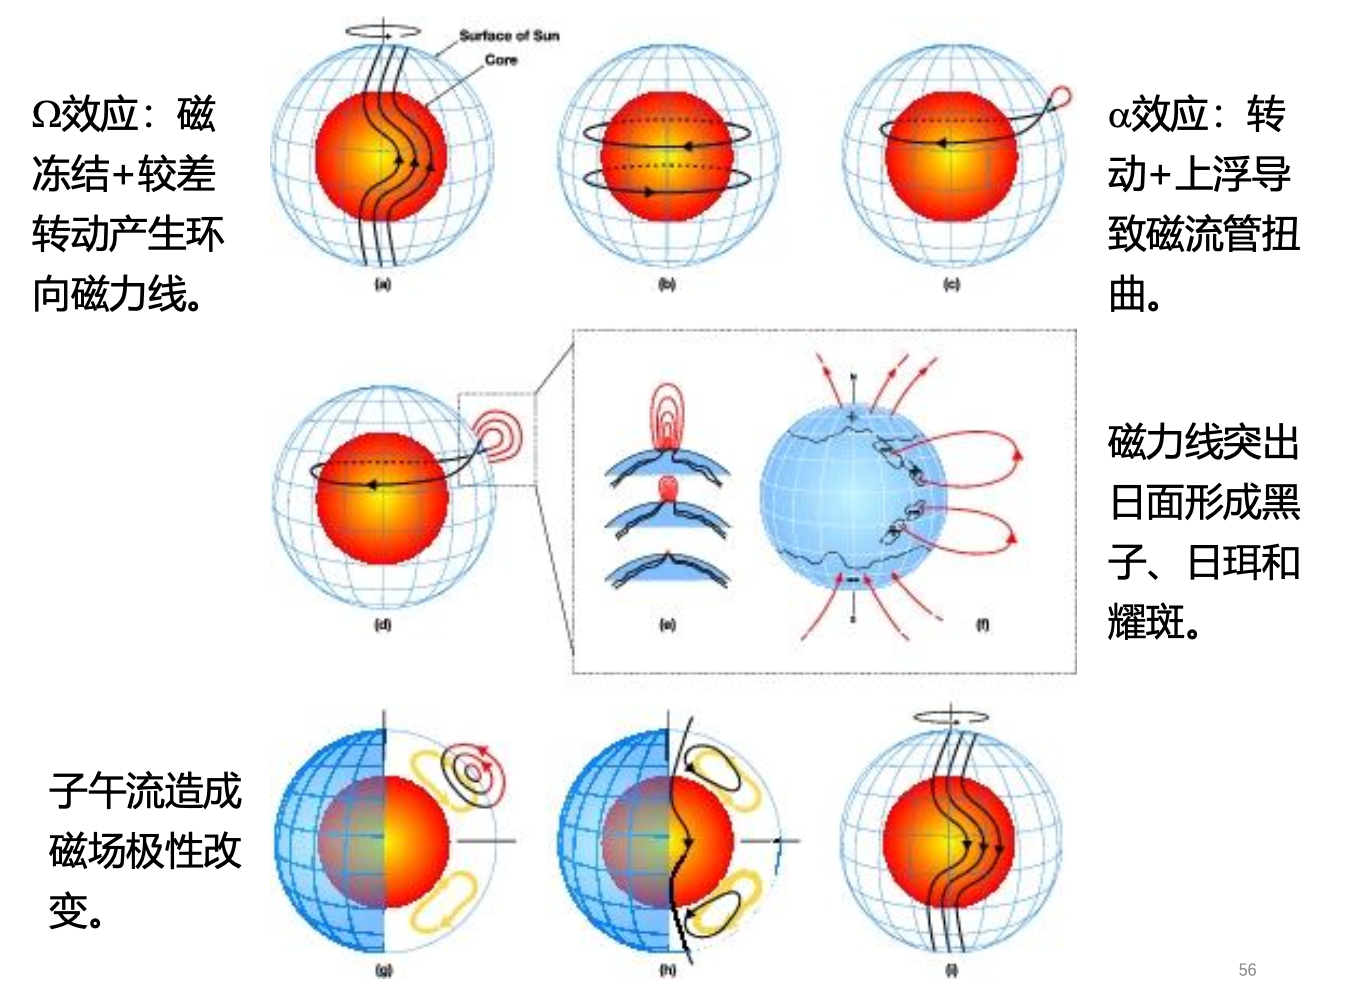
\includegraphics[width=6cm]{figures/figure1_1.png}
\end{minipage}
\begin{minipage}[t]{0.45\textwidth}
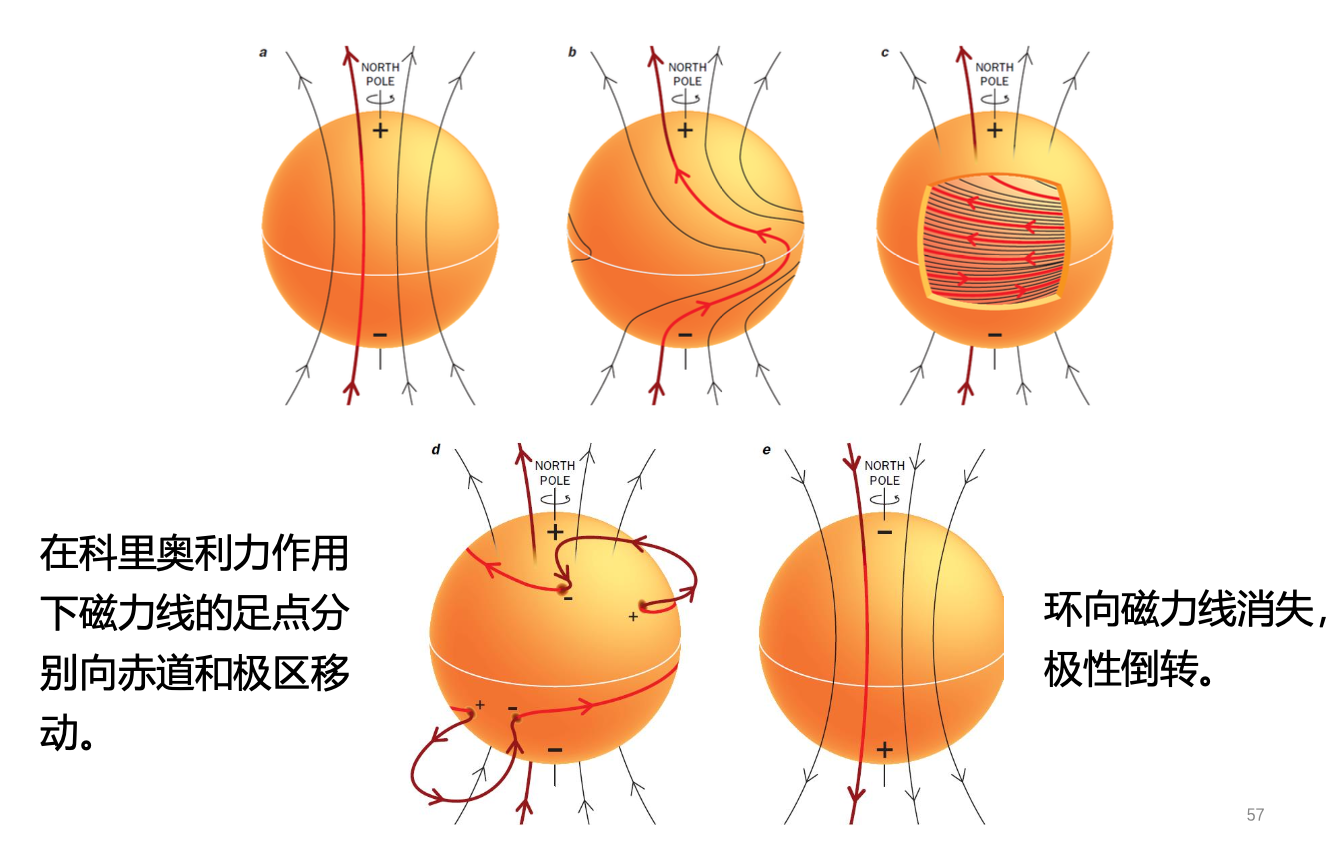
\includegraphics[width=6cm]{figures/figure1_2.png}
\end{minipage}
\captionsetup{justification=raggedright, singlelinecheck=false}
\caption{太阳磁力线的运动。}
\label{太阳磁力线的运动。}
\end{figure}

赤道式优点:天体的视运动可以很容易地利用赤经轴的匀速转动来补偿,视场的星像位置没有相对转动,在观测条件最好的天顶位置没有盲区。

赤道式缺点:承载量有限,望远镜的口径有限制,非对称式结构望远镜口径的极限是 $2.5\,\mathrm{m}$ 左右,对称式结构望远镜的口径一般不超过 $5\,\mathrm{m}$.

地平式优点:镜筒只在一个方向上承受弯矩的作用,承载重量大;作用在望远镜支臂上的力是不变的竖直向上的力,对望远镜的指向没有影响,回转半径小,可以使用小尺寸的圆顶或更为紧凑、跟随望远镜转动的观察室。望远镜的安装地点与当地的地理纬度无关。

地平式缺点:天顶盲区,在这个区域无法对天体进行跟踪观察,像场旋转。

黄道光 (Zodiacal Light): 位于地球上低纬度和中纬度地带的人于春季黄昏后在西方地平线上,或于秋季黎明前在东方地平线上所见到的淡弱的三角形光锥。黄道光沿着黄道向上伸展,可达地平线以上$30^{\circ}$左右。

黄道光的可见时间不长。春季黄昏后见到的黄道光,随着夜幕完全降临就逐渐消逝;秋季黎明前见到的黄道光,随着东方逐渐吐白就隐没于晨曦之中。

黄道光很暗弱,必须在良好的环境条件下才能有效地观测。春季黄昏后和秋季黎明前黄道面的空间方向恰好最接近于垂直地平面,所以这时黄道光就升得较高,容易看到。

在黄道上黄道光向太阳一直可以延伸到太阳的近旁,而在背太阳方向其亮度不断下降,然而离太阳 $135^{\circ}$ 左右,亮度反而有所增加,并在离太阳 $180^{\circ}$ 处又达到极大值,这就是对日照。

对日照的亮度更比黄道光暗弱,但与周围背景相比,却明显地明亮些。由于它十分微弱,几乎任何人为的光亮都足以使它相形见拙而无法观测。

对日照的成因一般倾向于是行星尘埃物质反射太阳光而形成的。

恒星基本参数测定:

2.1.3 半径

直接测量:

空间望远镜成像

地面望远镜干涉,光学望远镜的分辨率可以达到毫角秒的分辨率。

掩食法

结果:

超巨星 $100\sim1000R_\odot$

巨星	 $10\sim100R_\odot$

矮星	 $\sim R_\odot$

中子星 $\sim10^{-5}R_\odot$

2.1.6 质量

双星 (binary stars) 由在彼此引力作用下以椭圆轨道互相绕转的两颗恒星组成的双星系统。

银河系大部分的恒星(尤其是大质量恒星)位于双星和聚星系统中。

验证万有引力定律

→测量恒星质量

→研究恒星结构(形状、大小、大气)

→研究(特殊条件下的)恒星演化

→研究物质交流和吸积过程

利用开普勒第三定律
$$
\frac{\alpha^3}{T^2}=\frac{G}{4\pi^2}(M_1+M_2)
$$
将恒星质量测量转换为双星轨道半长径和周期测量,进而转换成对恒星位置和运动的测量、或者测量谱线频率变化,光度变化和轨道倾角。还需知道一颗恒星的质量和质量比。

目视双星 即望远镜分辨

天体测量双星 双星的一颗子星较暗无法观测到,但通过较亮子星的自行轨迹的变化可以推测其伴星的存在。

分光双星 谱线多普勒位移确定速度和倾角,这里可以加视向速度变化曲线 

食双星 相互交食 光变曲线 反映了温度比、轨道倾角和恒星的大小


\printbibliography
\end{document}